\documentclass{article}
\usepackage{amsmath}
\usepackage{graphicx}
\usepackage[colorlinks=true, linkcolor=blue, citecolor=black, backref=page]{hyperref}
\usepackage{lscape}
\usepackage{placeins}
\usepackage{listings}
\usepackage{xcolor}
\usepackage{float}
% Define custom colors
\definecolor{dkgreen}{rgb}{0,0.6,0}
\definecolor{gray}{rgb}{0.5,0.5,0.5}
\definecolor{mauve}{rgb}{0.58,0,0.82}

% Configure lstlisting settings for Python
\lstset{
  frame=tb,                      % Draw a frame at the top and bottom of the code block
  language=Python,               % Set the language to Python
  aboveskip=3mm,                 % Add space above the code block
  belowskip=3mm,                 % Add space below the code block
  showstringspaces=false,        % Do not display string spaces with special underlines
  columns=flexible,              % Allow flexible column spacing
  basicstyle={\small\ttfamily},  % Set the font style and size for code
  numbers=left,                  % Display line numbers on the left
  numberstyle=\tiny\color{gray}, % Style for line numbers
  keywordstyle=\color{blue},     % Style for keywords
  commentstyle=\color{dkgreen},  % Style for comments
  stringstyle=\color{mauve},     % Style for strings
  breaklines=true,               % Allow long lines to break
  breakatwhitespace=true,        % Break lines at whitespace if possible
  tabsize=4                      % Set tab size to 4 spaces
}


\begin{document}

\title{Task 4 -- NLO Lab Sheet 2}

\maketitle




\section*{Solution to 4(a) - Convergence Analysis of Steepest Descent with Armijo Line Search}



\section{Algorithm Implementation}

\subsection{Output}

\begin{figure}[H]
    \centering
    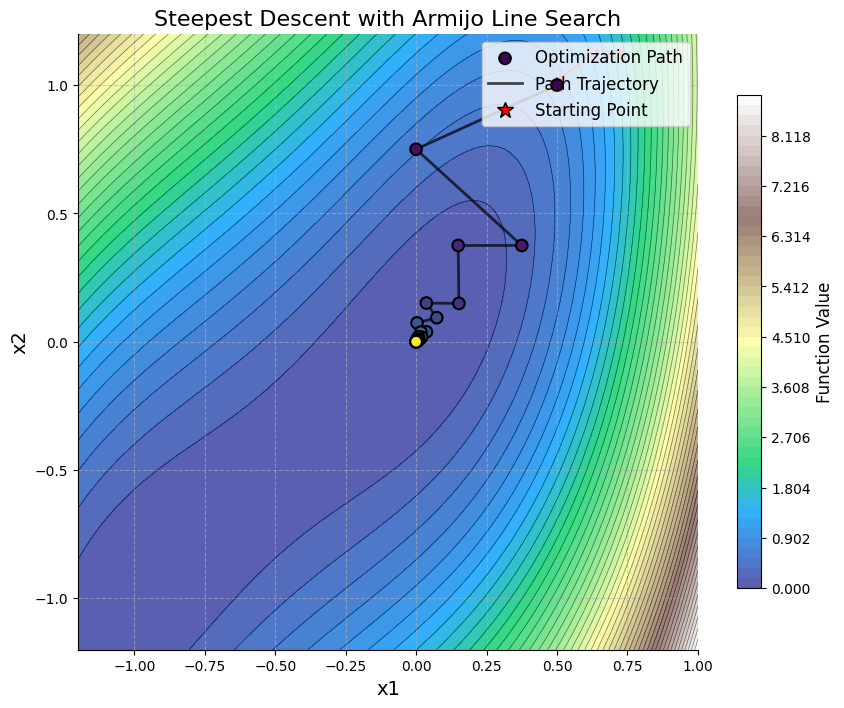
\includegraphics[width=1\textwidth]{Lab2_1.png}
    \caption{\textbf{\textit{Number of iterations = 27, Number of functional values = 99, $c_1 = 0.1$. The solution converges to $x^* = (0,0)$.}}}
    \label{lab21}
\end{figure}

\subsection{Python Code}
We can use the following code to obtain the ratios as asked in the question:
\begin{lstlisting}

import numpy as np

 Code of  LineSearchPlot.py

# Get the number of items in 'path' (assuming 'path' is a 2D NumPy array)
n_items, _ = path.shape

# Calculate the Euclidean norm  of each row in 'path'
norms = np.linalg.norm(path, axis=1)

# Determine the ratio of consecutive norms (from second to first norm itreatively)
ratios = norms[1:n_items] / norms[:-1]  



\end{lstlisting}


\subsection*{2. Analysis}
\textbf{
The value of $\|x_{k+1} - x^*\|/\|x_k- x^*\|$ keeps shifting  between 0.665 and 0.752}, revealing a zigzagging behavior in the descent which can be seen in Figure \ref{lab21}. The alternating pattern suggests consistent behavior despite inexact searches with the solution as $x = (0,0)$. 

We therefore have a \textbf{linear rate of convergence with $r = 0.75$}.\\

Hessian at the solution is given by:
\[
\nabla^2f(x^*) = \begin{bmatrix} 4 & -2 \\ -2 & 2 \end{bmatrix}
\]

\textbf{Eigenvalue computation}:
\begin{align*}
\det(\nabla^2f(x^*) - \lambda I) &= 0 \text{ is the characteristic equation} \\
\lambda^2 - 6\lambda + 4 &= 0 \\
\lambda_1 \approx  5.23607\\
\lambda_2 \approx  0.76393
\end{align*}


Both eigenvalues are positive, and the Hessian matrix is  hence \textbf{positive definite}.


The theoretical convergence rate:
\[
r = \frac{\lambda_1-\lambda_2}{\lambda_1+\lambda_2} \approx 0.74535  
\]
\[r^2 = 0.55555\]
which is smaller than the observed rate. 

But, \textbf{Theorem 3.4 in Nocedal and Wright upper bounds the ratio of function values, not the $x$- argument values}.
The functional value ratio, still alternates between $0.34$ and $0.73$. The theoretical rate is still less in magnitude, but the bound holds strictly for exact line searches, which may not be applicable in this case but it still works nonetheless as we can see the zigzagging behavior.

\textbf{ There is agreement to some extent but there is definitely not a strict agreement. 
}


\section*{Solution to 4(b) - Analysis of Armijo Line Search with \( c_1 = 0.9 \)}


With \( c_1 = 0.9 \), the Armijo line search \textbf{trajectory follows the steepest continuous descent path taking many smaller continuous steps(Figure \ref{lab22}) }instead of larger direct and discrete steps(Figure \ref{lab23}). The Armijo condition,

\textbf{\[
f(x_k + \alpha d_k) \leq f(x_k) + c_1\alpha\nabla f(x_k)^\top d_k,
\]
ensures that the function value reduction is at least 90\% of the linear approximation of the descent, with for some flexibility in step selection}. Since the linear approximation is only accurate for small \( \alpha \), larger steps typically fail this criterion, leading to numerous smaller steps. 


In contrast, the the exact line search, which generally requires \( c_1 \leq 0.5 \), would accept the iterations or steps that Armijo with \( c_1 = 0.9 \) would strictly eradicate, leading to a path of optimization that is entirely different. The method ensures convergence, but it is inefficient as it takes a large number of small steps, making it computationally expensive despite generating a smoother trajectory.

\begin{figure}[H]
    \centering
    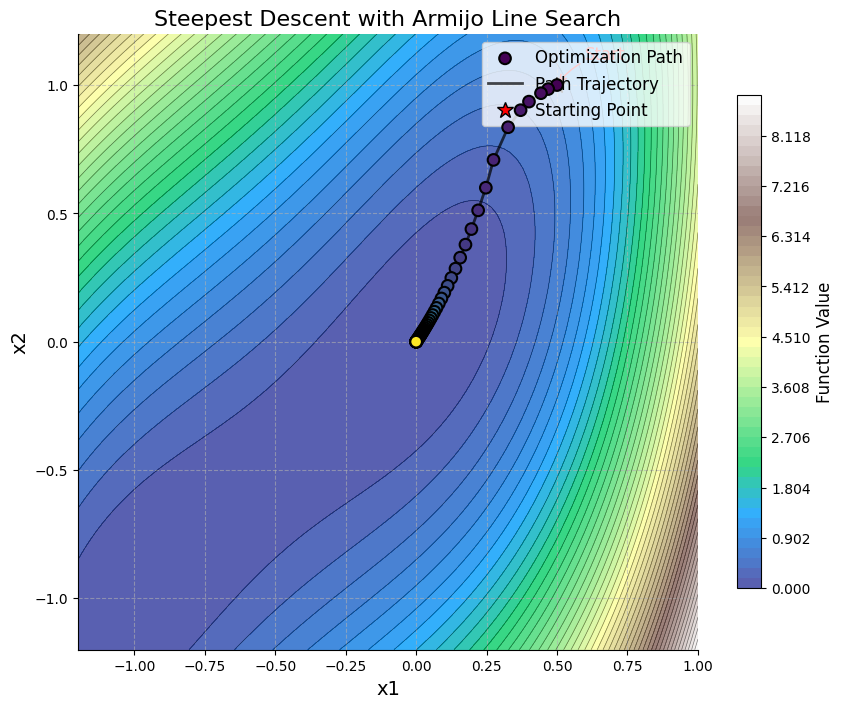
\includegraphics[width=1\textwidth]{Lab2_2.png}
    \caption{\textbf{\textit{Number of iterations = 60, Number of functional values = 288, $c_1 = 0.9$.}}}
    \label{lab22}
\end{figure}

\begin{figure}[H]
    \centering
    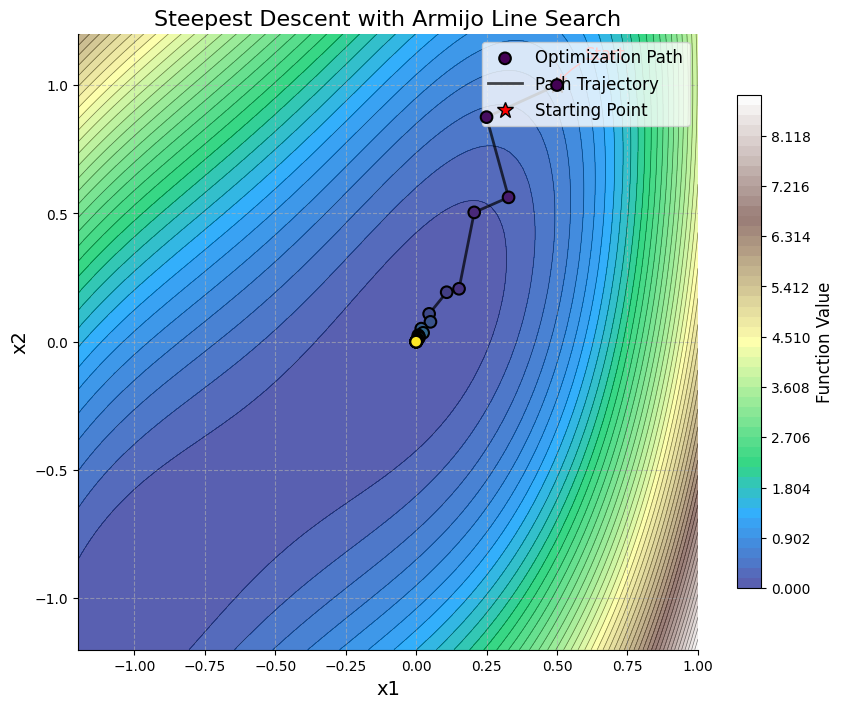
\includegraphics[width=1\textwidth]{Lab2_3.png}
    \caption{\textbf{\textit{Number of iterations = 27, Number of functional values = 101, $c_1 = 0.5$ }}}
    \label{lab23}
\end{figure}
\end{document}

